\documentclass[a4paper, 12pt]{article}

\usepackage[portuges]{babel}
\usepackage[utf8]{inputenc}
\usepackage[margin=1.2in]{geometry}
\usepackage{amsmath}
\usepackage{indentfirst}
\usepackage{graphicx}
\usepackage{datetime}
\usepackage{enumerate}
\renewcommand{\baselinestretch}{1.5}

\emergencystretch 1em%

\begin{document}

\section*{Parte I - Atividades teóricas}

\subsection*{Exercício 1}

\begin{enumerate}[a)]
\item
$P(A^C) = 1 - P(A) = 1 - \frac{1}{3} = \frac{2}{3}$

\item
$P(A^C \cup B) = P(A^C) + P(B) - P(A^CB) = P(A^C) + P(B) - (P(B) - P(AB)) = P(A^C) + P(AB) = \frac{2}{3} + \frac{1}{6} = \frac{5}{6}$

\item
$P(A \cup B^C) = P(A) + P(B^C) - P(AB^C) = P(B^C) + P(AB) = (1 - P(B)) + P(AB) = (1 - \frac{1}{4}) + \frac{1}{6} = \frac{5}{12}$

\item
$P(AB^C) = P(A) + P(B^C) - P(A \cup B^C) = \frac{1}{3} + \frac{3}{4} - \frac{5}{12} = \frac{8}{12}$

\item
$P(A^C \cup B^C) = P(A^C) + P(B^C) - P(A^CB^C) = \frac{2}{3} + \frac{3}{4} - \frac{5}{6} = \frac{7}{12}$

\end{enumerate}

\subsection*{Exercício 2}

\begin{enumerate}[a)]
\item
$$
    F_X(x) = P(X \leq x) = \int\limits_{-\infty}^x f_X(\xi) d\xi = \int\limits_{-\infty}^x \frac{1}{2} d\xi = \left[ \frac{1}{2}\xi \right]^x_0 = \frac{1}{2} x, \forall X \in [0, 2]
$$

\item
$E\{X\} = \int\limits_{-\infty}^{\infty} xf_X(x)dx = \int\limits_0^2 \frac{1}{2}x dx = \left[\frac{x^2}{4}\right]^2_0 = 1$

$E\{X^2\} = \int\limits_{-\infty}^{\infty} x^2f_X(x)dx = \int\limits_0^2 \frac{1}{2}x^2 dx = \left[\frac{x^3}{6}\right]^2_0 = \frac{4}{3}$

$E\{X^3\} = \int\limits_{-\infty}^{\infty} x^3f_X(x)dx = \int\limits_0^2 \frac{1}{2}x^3 dx = \left[\frac{x^4}{8}\right]^2_0 = 2$
\end{enumerate}

\subsection*{Exercício 3}

\begin{enumerate}[a)]
\item
$X_2$, pois quanto mais próximo da distribuição uniforme, mais difícil é acertar o resultado de um evento aleatório "chutando um valor", ou seja, a variável aleatória $X_2$ carrega mais informação que a variável aleatória $X_1$, pois neste último eu poderia supor que o resultado será sempre 3 com uma taxa de acertos de 40\% contra uma taxa de acertos de 25\% para qualquer valor estimado para $X_2$ se não tivermos nenhuma informação \em a priori\em .


\item
$H(X_1) = - \sum\limits_x p(X_1)log_2[p(X_1)] = -[0,1(-3,32) + 0,2(-2,32) + 0,3(-1,74) + 0,4(-1,32)] = 1,85$

$H(X_2) = - \sum\limits_x p(X_2)log_2[p(X_2)] = - [0,25 (-2) + 0,25 (-2) + 0,25 (-2) + 0,25(-2)] = 2$


\item
$D(P_1 || P_2) = \sum\limits_x p(X_1)log_2\left[\frac{p(X_1)}{p(X_2)}\right] = 0,1(-1,32) + 0,2(-0,32) + 0,3(-0,26) + 0,4(-0,68) = -0,54$

$D(P_2 || P_1) = \sum\limits_x p(X_2)log_2\left[\frac{p(X_2)}{p(X_1)}\right] = 0,25(1.32 +  0.32 - 0.26 -0.68) = 0,18$

\end{enumerate}

\subsection*{Exercício 4}

\begin{enumerate}[a)]
\item
$\mu_{ML} = arg max_\theta p(x|\mu) = arg max_\theta log[p(x|\mu)] = arg max_\theta \frac{p(x\mu)}{p(\mu)} = x$

\item
$\mu_{ML} = arg max_\theta p(\mathbf{x}|\mu) = arg ax_\theta log[p(\mathbf{x}|\mu)] = arg max_\theta \sum\limits_{k=1}^{N} log[p(x_K|\mu)] = arg max_\theta \sum \limits_{k=1}^{N} log\left [ \frac{p(x_K\mu)}{p(\mu)}\right ] $

\item

\end{enumerate}

\newpage

\section*{Parte II - Atividade computacional}

\subsection*{Solução fechada com MMQ}

\begin{figure}[h!]
  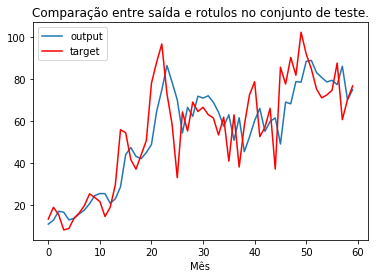
\includegraphics{images/raw.png}
    \caption{Saída prevista pelo modelo (azul) em comparação com valores reais dos últimos 5 anos (60 meses).}
\end{figure}

\subsection*{Solução fechada com MMQ}

\begin{figure}[h!]
  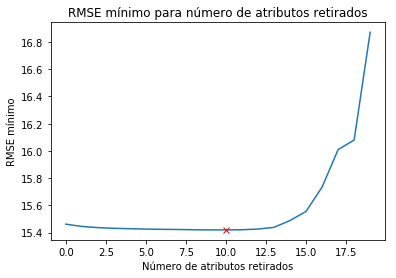
\includegraphics{images/backward.png}
    \caption{Saída prevista pelo modelo (azul) em comparação com valores reais dos últimos 5 anos (60 meses).}
\end{figure}

\begin{figure}[h!]
  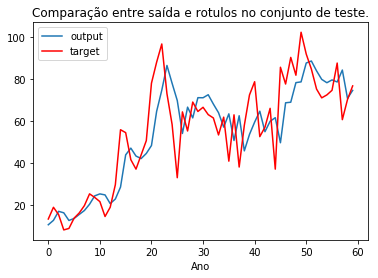
\includegraphics{images/wrapper.png}
    \caption{Saída prevista pelo modelo (azul) em comparação com valores reais dos últimos 5 anos (60 meses).}
\end{figure}

\subsection*{Solução fechada com MMQ}

\begin{figure}[h!]
  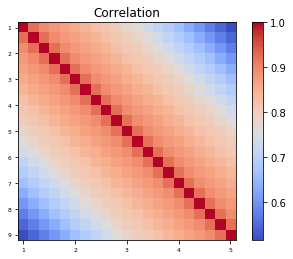
\includegraphics{images/corr.png}
    \caption{Saída prevista pelo modelo (azul) em comparação com valores reais dos últimos 5 anos (60 meses).}
\end{figure}

\begin{figure}[h!]
  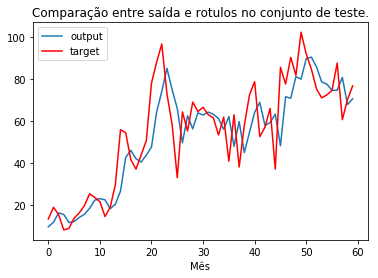
\includegraphics{images/filter.png}
    \caption{Saída prevista pelo modelo (azul) em comparação com valores reais dos últimos 5 anos (60 meses).}
\end{figure}

\begin{figure}[h!]
  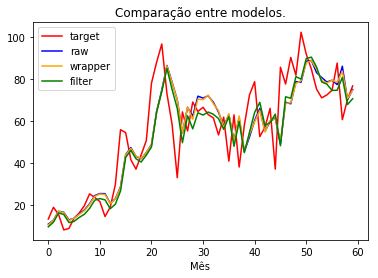
\includegraphics{images/comparison.png}
    \caption{Saída prevista pelo modelo (azul) em comparação com valores reais dos últimos 5 anos (60 meses).}
\end{figure}

\end{document}
